\documentclass[conference]{IEEEtran}
\IEEEoverridecommandlockouts
% The preceding line is only needed to identify funding in the first footnote. If that is unneeded, please comment it out.
\usepackage{cite}
\usepackage{amsmath,amssymb,amsfonts}
%\usepackage{algorithmic}
\usepackage{graphicx}
\usepackage{textcomp}
\usepackage{xcolor}
\def\BibTeX{{\rm B\kern-.05em{\sc i\kern-.025em b}\kern-.08em
    T\kern-.1667em\lower.7ex\hbox{E}\kern-.125emX}}
\begin{document}

\title{Simple Wireless Link Simulations\\
%{\footnotesize \textsuperscript{*}Note: Sub-titles are not captured in Xplore and
%should not be used}
%\thanks{Identify applicable funding agency here. If none, delete this.}
}

\author{\IEEEauthorblockN{ Armaan Kohli}
\IEEEauthorblockA{\textit{Department of Electrical Engineering} \\
\textit{The Cooper Union for the Advancement of Science and Art}\\
New York City, United States \\
kohli@cooper.edu}}
%\and
%\IEEEauthorblockN{2\textsuperscript{nd} Given Name Surname}
%\IEEEauthorblockA{\textit{dept. name of organization (of Aff.)} \\
%\textit{name of organization (of Aff.)}\\
%City, Country \\
%email address or ORCID}
%\and
%\IEEEauthorblockN{3\textsuperscript{rd} Given Name Surname}
%\IEEEauthorblockA{\textit{dept. name of organization (of Aff.)} \\
%\textit{name of organization (of Aff.)}\\
%City, Country \\
%email address or ORCID}
%\and
%\IEEEauthorblockN{4\textsuperscript{th} Given Name Surname}
%\IEEEauthorblockA{\textit{dept. name of organization (of Aff.)} \\
%\textit{name of organization (of Aff.)}\\
%City, Country \\
%email address or ORCID}
%\and
%\IEEEauthorblockN{5\textsuperscript{th} Given Name Surname}
%\IEEEauthorblockA{\textit{dept. name of organization (of Aff.)} \\
%\textit{name of organization (of Aff.)}\\
%City, Country \\
%email address or ORCID}
%\and
%\IEEEauthorblockN{6\textsuperscript{th} Given Name Surname}
%\IEEEauthorblockA{\textit{dept. name of organization (of Aff.)} \\
%\textit{name of organization (of Aff.)}\\
%City, Country \\
%email address or ORCID}
%}

\maketitle

\begin{abstract}
We simulate three different wireless channels to demonstrate understanding of the fundamentals of communication theory. 

\end{abstract}

\begin{IEEEkeywords}
wireless link simulations, turbo codes, adaptive equalization 
\end{IEEEkeywords}

\section{Introduction}
We simulate three different wireless links. First, we verify simulating 4QAM and 16QAM simulations match theoretical bit error rate (BER) curves. Next, we design an adaptive equalizer to mitigate inter-symbol-interference over a wireless channel and achieve a BER less than $10^{-4}$ at 12dB signal-to-noise ratio (SNR) for BPSK. Finally, we use error correcting codes to maximize bit rate and achieve a BER less than $10^{-6}$ at 12dB SNR.

\section{4QAM \& 16QAM Performance}
We were able to successfully match theoretical performance for both 4 and 16-ary QAM schemes over additive white Gaussian noise (AWGN) channels. 

We simulated performance by computing the bit error rate for a single 1000 symbol packet, averaged over 10 iterations. BER curves and constellation diagrams for 4QAM can be seen in Fig. \ref{4ber} and \ref{4star}. BER curves and constellation diagrams for 16QAM can be seen in Fig. \ref{16ber} and \ref{16star}
\subsection{4QAM}
\begin{figure}[htbp]
\centerline{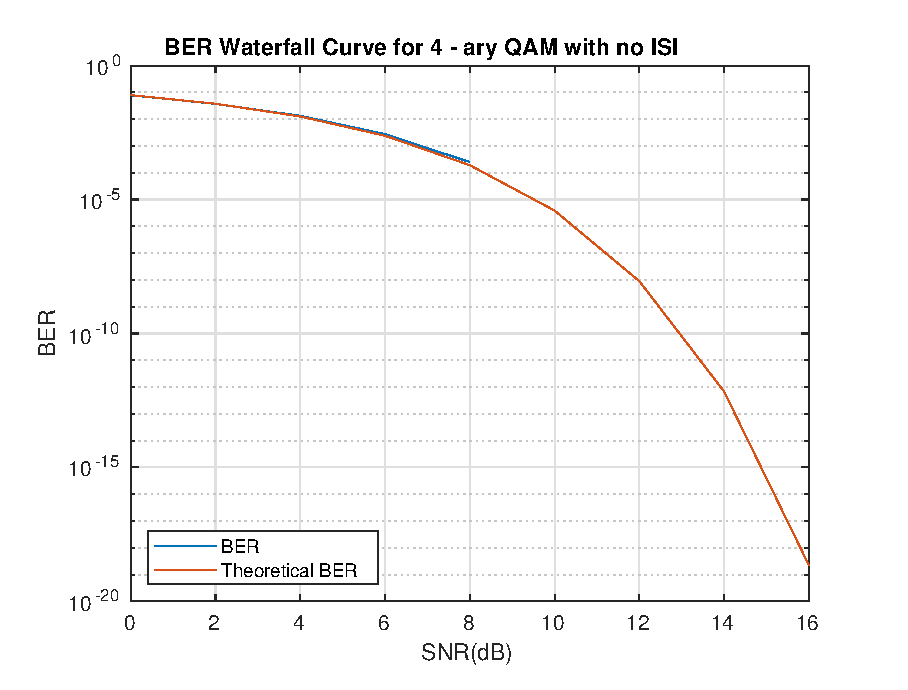
\includegraphics[scale=.5]{./media/4qam.eps}}
\caption{BER Curve for 4QAM over an AWGN channel}
\label{4ber}
\end{figure}
\begin{figure}[htbp]
\centerline{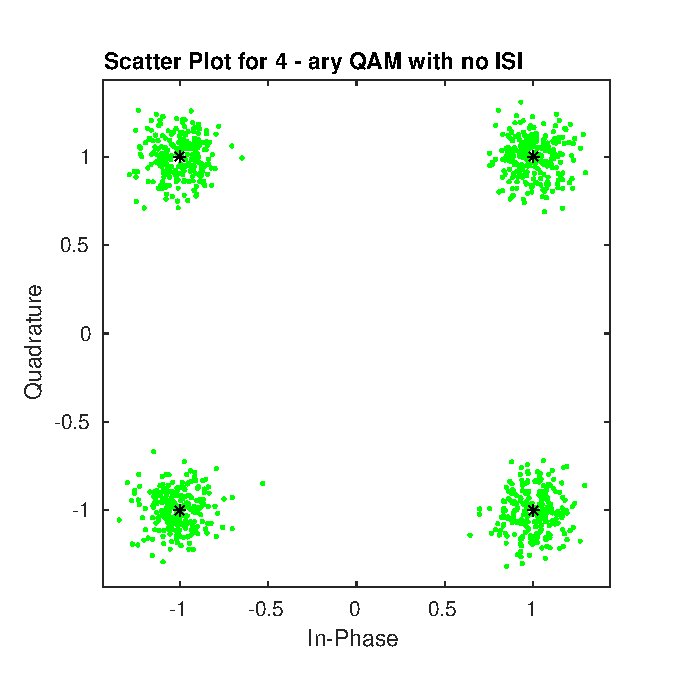
\includegraphics[scale=.5]{./media/4qam_scatter.eps}}
\caption{4QAM constellation}
\label{4star}
\end{figure}
\subsection{16QAM}
\begin{figure}[htbp]
\centerline{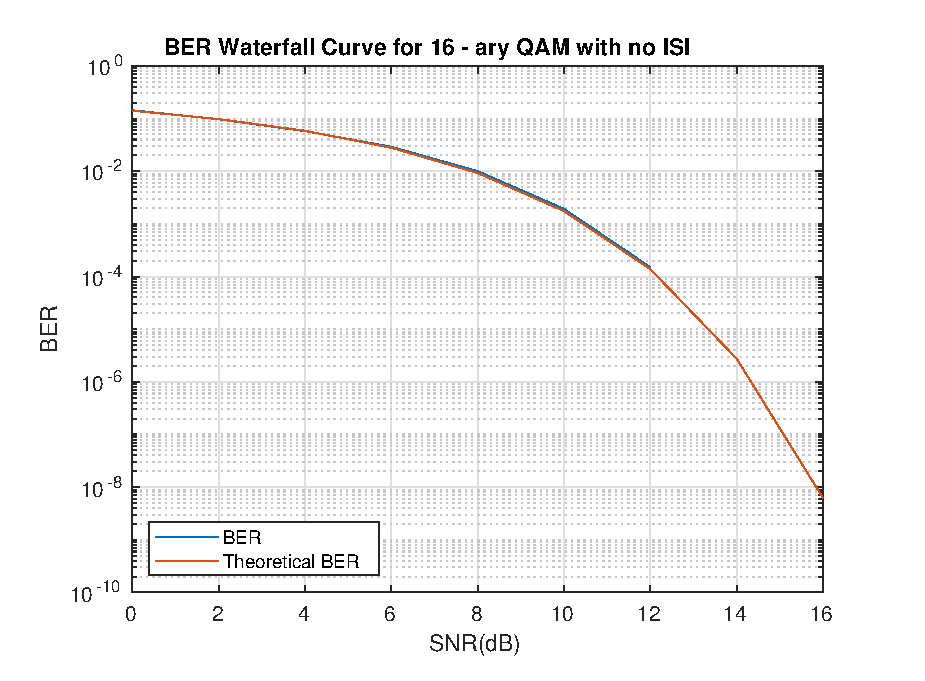
\includegraphics[scale=.5]{./media/16qam.eps}}
\caption{BER Curve for 16QAM over an AWGN channel}
\label{16ber}
\end{figure}
\begin{figure}[htbp]
\centerline{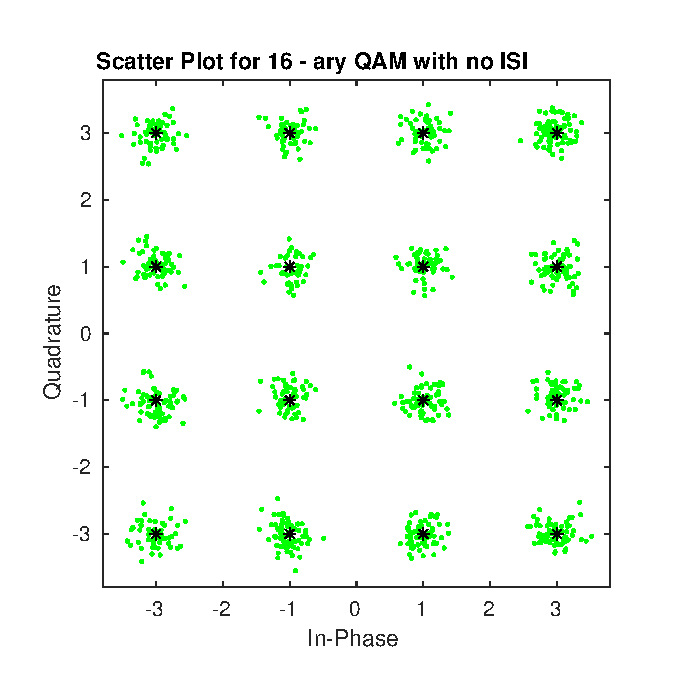
\includegraphics[scale=.5]{./media/16qam_scatter.eps}}
\caption{16QAM constellation}
\label{16star}
\end{figure}

\section{Equalizing a Moderate ISI Channel}
Next, we attempt to equalize a frequency selective channel that introduces ISI, using a BPSK modulation scheme. We attempted several different adaptive filtering algorithms in an attempt to equalize the channel. Generally speaking, we found RLS based algorithms difficult to stabilize, and linear equalizers tended to require long training sequences. We found that we achieved the best performance using a decision feedback equalizer (DFE) with a signed-LMS algorithm.

We simulated the channel with $100,000$ symbols in order to ensure we met the performance specification of a BER less than $10^{-4}$ at 12dB, averaged over five iterations. 
\begin{figure}[htbp]
\centerline{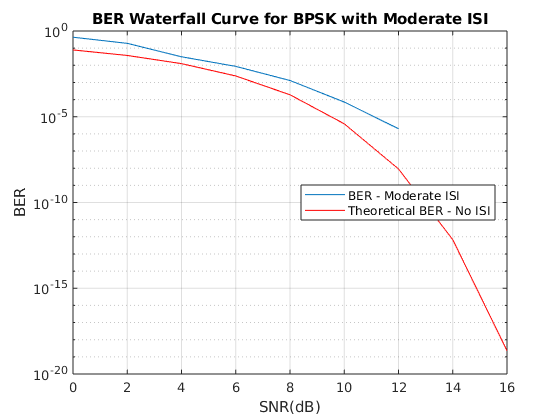
\includegraphics[scale=.4]{./media/bpsk.png}}
\caption{BER Curve for BPSK over a frequency selective channel}
\label{16ber}
\end{figure}
\begin{figure}[htbp]
\centerline{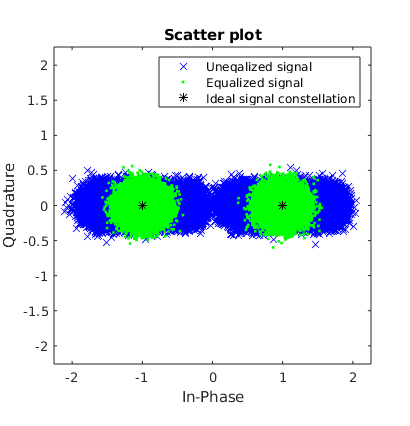
\includegraphics[scale=.4]{./media/bpsk_scatter.png}}
\caption{BPSK constellation}
\label{16star}
\end{figure}
We were able to successfully meet the specification, achieving a BER of approximately $10^{-6}$ at 12dB SNR.
\section{Maximizing Bit Rate via Coding}
Finally, we attempted to further improve the performance of our wireless communication system by introducing error control codes. In order to maximize bit rate while still achieving the $10^{-6}$ BER requirement at 12dB SNR, we decided to increase the order of modulation and use turbo codes. 

We used 16QAM and a code rate of $\frac{2}{3}$ for the turbo codes. We generated the BER curve in Fig. \ref{turbo} using the standard 1000 symbol packet, averaged over five iterations. 
\begin{figure}[htbp]
\centerline{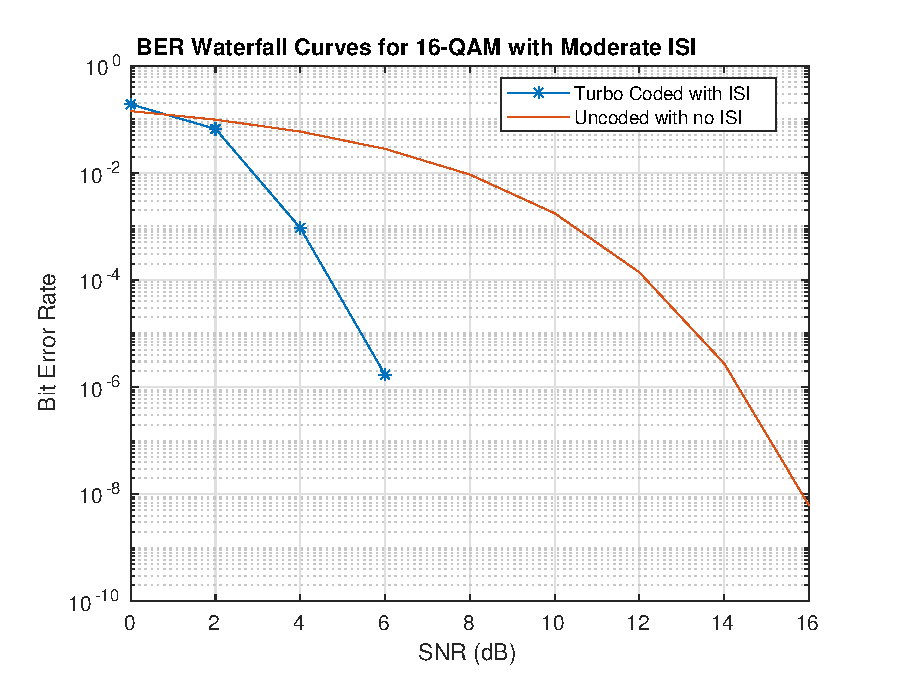
\includegraphics[scale=.55]{./media/turbo.eps}}
\caption{BER curve for 16QAM w/ using turbo error control codes}
\label{turbo}
\end{figure}

\section{Conclusion}
We were able to successfully demonstrate understanding of communication theory fundamentals. We simulated AWGN and frequency selective channels, and corrected ISI both via adaptive equalization and error correcting codes.

%\section*{References}
%
%Please number citations consecutively within brackets \cite{b1}. The 
%sentence punctuation follows the bracket \cite{b2}. Refer simply to the reference 
%number, as in \cite{b3}---do not use ``Ref. \cite{b3}'' or ``reference \cite{b3}'' except at 
%the beginning of a sentence: ``Reference \cite{b3} was the first $\ldots$''
%
%Number footnotes separately in superscripts. Place the actual footnote at 
%the bottom of the column in which it was cited. Do not put footnotes in the 
%abstract or reference list. Use letters for table footnotes.
%
%Unless there are six authors or more give all authors' names; do not use 
%``et al.''. Papers that have not been published, even if they have been 
%submitted for publication, should be cited as ``unpublished'' \cite{b4}. Papers 
%that have been accepted for publication should be cited as ``in press'' \cite{b5}. 
%Capitalize only the first word in a paper title, except for proper nouns and 
%element symbols.
%
%For papers published in translation journals, please give the English 
%citation first, followed by the original foreign-language citation \cite{b6}.
%
%%\begin{thebibliography}{00}
%%\bibitem{b1} G. Eason, B. Noble, and I. N. Sneddon, ``On certain integrals of Lipschitz-Hankel type involving products of Bessel functions,'' Phil. Trans. Roy. Soc. London, vol. A247, pp. 529--551, April 1955.
%%\bibitem{b2} J. Clerk Maxwell, A Treatise on Electricity and Magnetism, 3rd ed., vol. 2. Oxford: Clarendon, 1892, pp.68--73.
%%\bibitem{b3} I. S. Jacobs and C. P. Bean, ``Fine particles, thin films and exchange anisotropy,'' in Magnetism, vol. III, G. T. Rado and H. Suhl, Eds. New York: Academic, 1963, pp. 271--350.
%%\bibitem{b4} K. Elissa, ``Title of paper if known,'' unpublished.
%%\bibitem{b5} R. Nicole, ``Title of paper with only first word capitalized,'' J. Name Stand. Abbrev., in press.
%%\bibitem{b6} Y. Yorozu, M. Hirano, K. Oka, and Y. Tagawa, ``Electron spectroscopy studies on magneto-optical media and plastic substrate interface,'' IEEE Transl. J. Magn. Japan, vol. 2, pp. 740--741, August 1987 [Digests 9th Annual Conf. Magnetics Japan, p. 301, 1982].
%%\bibitem{b7} M. Young, The Technical Writer's Handbook. Mill Valley, CA: University Science, 1989.
%%\end{thebibliography}

\end{document}
